\documentclass{article}
\usepackage{changepage}
\usepackage{float}
\usepackage{noah}
\usepackage{{appendix}}

\usepackage[font=small,labelfont=bf]{caption} 
%% Stuff for inserting code into document
\usepackage{listings}
\usepackage{color}

\definecolor{dkgreen}{rgb}{0,0.6,0}
\definecolor{gray}{rgb}{0.5,0.5,0.5}
\definecolor{mauve}{rgb}{0.58,0,0.82}

\lstset{frame=tb,
  language=Python,
  aboveskip=3mm,
  belowskip=3mm,
  showstringspaces=false,
  columns=flexible,
  basicstyle={\small\ttfamily},
  numbers=none,
  numberstyle=\tiny\color{gray},
  keywordstyle=\color{blue},
  commentstyle=\color{dkgreen},
  stringstyle=\color{mauve},
  breaklines=true,
  breakatwhitespace=true,
  tabsize=3
}

\author{Noah Jeffrey Blair}
\title{Vibrations and Heat Diffusion on the Unit Disc}
\begin{document}
\maketitle
\begin{abstract}
  The method of eigenfunction expansion is developed and demonstrated for solutions to the Helmholtz equation on the unit disc. Through this method, Greens' functions for the wave and heat equation are generated and particular solutions are analyzed, to show the variety of dynamics possible within the realm of partial differential equations.
\end{abstract}
\tableofcontents
\newpage
\section{Introduction}
Partial differential equations (PDEs) are a natural extension to  ordinary differential equations, in that they describe systems that can vary with respect to multiple variables, traditionally position and time. Two fundamental PDEs are the heat and wave equations. Both of these involve the Laplace operator, defined in the following way:
\begin{equation}
  \lapl f := \dive(\grad f)
\end{equation}
Note, that it is sometimes written as $\nabla^2 f$. Due to its nature as being the divergence of the gradient of some function, it is a natural generalization to the second derivative with respect to a position variable, and can be written in the following way:
\begin{equation}
  \lapl f = \pder{^2 f}{x^2}+\pder{^2 f}{y^2}= \pder{^2 f}{r^2}+\frac{1}{r}\pder{f}{r}+\frac{1}{r^2}\pder{^2 f}{\phi^2}
\end{equation}
where $(x,y)$ represent a point in Cartesian coordinates and $(r,\phi)$ represents a point in polar coordinates. Solutions to Laplace's equation $\lapl u = 0$ are known as harmonic functions, and are of particular interest in both pure and applied mathematics.\\
This operator is used regularly in the description of many dynamical systems, including wave propagation, heat diffusion, and many other PDEs.\\
The wave equation, as the name suggests, describes how waves propagate through a given domain. Consider a string with fixed ends that is allowed to vibrate. The motion that we are interested in is transverse motion, so we consider the forces in a direction normal to the line. Newton's second law tells us the following for the dynamics of a small bit of mass on a string:
\begin{equation}
    F_{net}=dm\cdot a=\lambda dx \cdot a
\end{equation}
where $\lambda$ is the linear mass density, and $a$ is the vertical acceleration of the string. If we raise part of the string near this point so that the angle the string makes between these two points is $\theta$, then the force is:
\begin{equation}
    F_{net}=T \sin(\theta + d\theta)-T \sin(\theta)=T\cos(\theta)d\theta
\end{equation}
where $T$ is the tension in the rope. If we assume small enough displacements, we can approximate $\cos\theta\approx 1$ and write $d\theta= (\partial\theta/\partial x) dx$. Since we are assuming small displacements, we can say that the angle $\theta$ is the slope of the string. We will write the displacement of the string as $u=u(x,t)$, and say that this function must satisfy the following equation:
\begin{equation}\pder{^2 u}{t^2}= \frac{T}{\lambda}\pder{^2 u}{x^2}=c^2 \pder{^2 u}{x^2}\end{equation}
We are introducing the constant $c$ which is the speed of propagation on the string. This can be absorbed into our time variable, by redefining our unit of time. For higher spatial dimensions, the second partial derivative with respect to $x$ is replaced with the Laplacian, so the general wave equation is:
\begin{equation}
  \boxed{
    \lapl u =\pder{^2 u}{t^2}
  }
\end{equation}
We see that when the vibrating object is not accelerating, the Laplacian is zero, which means that the steady state behavior of the wave equation is a harmonic function. As we will see later, solutions to the wave equation oscillate about harmonic functions.\\
The heat equation has a similar form as the wave equation, but with very different dynamics. The general assumption behind the heat equation is conservation of energy. This conservation law is formulated in terms of a continuity equation:
\begin{equation}
  \pder{u}{t}+\dive \vect{J}=0
\end{equation}
Here $u$ is the energy density, and $\vect{J}$ is the energy flux. This equation states that if energy is flowing into a region, then the energy density must be increasing. In order to find the energy flux, we use Newton's Law of cooling which states that the energy flow is proportional to the temperature difference between two regions. This can be formulated in the following way:
\begin{equation}
  \vect{J}=-\sigma\grad u
\end{equation}
where $\sigma$ is the thermal conductivity. The reason for using the energy gradient instead of the temperature gradient in this equation is that temperature is just a useful method for defining the energy. Using this, we may write the heat equation as:
\begin{equation}
  \boxed{
    \lapl u = \pder{u}{t}
  }
\end{equation}
Here we have absorbed the thermal conductivity into our definition of time. The interesting part of this equation is that it can be used to describe diffusive processes as well. In fact it can be used to describe many systems that do not violate the first and second law of thermodynamics. The first of these states energy conservation, and the second states that the entropy of a system must increase. This second law is one of the few that does depend on the direction of time. This is why the heat equation is not symmetric in the spatial and temporal variables, whereas the wave equation is.\\
This system has harmonic solutions whenever the system is not changing in time. Therefore, we see that in time, the solution tends towards a harmonic solution. It is for this reason that solutions to Laplace's equations describe steady state temperature distributions.\\
In order to analyze the different types of solutions these equations provide, as well as some general methods for solving PDEs, we will solve both of these equations on the unit disc $B^2$ with the boundary condition that the function must vanish at the boundary. Similar to the case for ODEs, we must also provide initial conditions. Since the heat equation is first order in time, we only need to know the initial heat distribution $u(r,\phi,0)=u_o(r,\phi)$. The wave equation is second order in time, so we must supply both the initial displacement of the circular membrane, $u(r,\phi,0)=u_o(r,\phi)$, and the initial velocity of $\der{t} u(r,\phi,0)=\dot{u}_o(r,\phi)$. Together with the boundary data, these conditions uniquely define a solution to the differential equation.
\section{Separation of Variables}
To begin solving these equations, we will employ a method known as separation of variables. In this we assume that the solution can be written as the product of single-variable functions. Since these are both functions of position and time, we assume a solution $u(r,\phi,t)=\psi(r,\phi)\chi(t)$. If we insert this into the heat equation, and divide by $u(r,\phi,t)$ we obtain the following:
\begin{equation}
  \frac{\lapl \psi}{\psi} = \frac{1}{\chi(t)}\dder{\chi}{t}
\end{equation}
The left-hand side is just a function of the spatial variables, while the right-hand side is just a function of time. This means that the two sides are independent of each other, and therefore must be equal to a constant. For reasons that will be clear later on, I will use $-k^2$ as the constant. This leaves us with two differential equations:
\begin{equation}
  \begin{matrix}
    \lapl\psi+k^2\psi=0\\
    \dot{\chi}=-k^2 \chi
  \end{matrix}
\end{equation}
We can easily solve the time equation to obtain:
\begin{equation}
  \chi_{\mathrm{heat}}(t)=\exp(-k^2 t)
\end{equation}
Any constants of integration may be absorbed into $\psi(r,\phi)$. If we follow this same procedure for the wave equation, we are left with the two separated differential equations:
\begin{equation}
  \begin{matrix}
    \lapl\psi+k^2\psi=0\\
    \ddot{\chi}=-k^2 \chi
  \end{matrix}
\end{equation}
Again the time component can be easily solved, to give the following solution:
\begin{equation}
  \chi_{\mathrm{wave}}=A\cos(kt)+B\sin(kt)
\end{equation}
It is important to notice that for both of these equations, the spatial part is the same. Given that we are using the same boundary conditions for both equations, solving this equation will provide us with solutions to both the wave and heat equation.
\section{The Helmholtz Equation}
The above differential equation:
\begin{equation}
  \lapl \psi+k^2\psi=0
\end{equation}
is known as the Helmholtz equation, and it describes the eigenvalues and eigenfunctions of the Laplacian on the unit disc. Recall that an eigenvalue equation is one where:
\begin{equation}
  \mc{L}v = \lambda v
\end{equation}
where $\mc{L}$ is a linear operator, $v$ is an eigenvector, and $\lambda$ is an eigenvalue. In the context of differential operators, the eigenvectors are referred to as eigenfunctions.\\
Given our boundary data, the eigenfunctions will be ones that satisfy the following equations:
\begin{equation}
  \boxed{
    \begin{matrix}
      \lapl \psi+k^2\psi=0 \\ 
      \psi(1,\phi) = 0
    \end{matrix}
  }
\end{equation}
In order to solve this equation, we again separate the variables, now assuming that $\psi(r,\phi)=f(r)g(\phi)$. If we insert this into the Helmholtz equation and divide by $\psi$ we obtain:
\begin{equation}
  \frac{1}{f(r)}\left[r^2 \dder{^2 f}{r^2} + r \dder{f}{r}+k^2 r^2\right] = -\frac{1}{g(\phi)}\dder{^2 g}{\phi^2} = n^2
\end{equation}
Again the left-hand side is a function of $r$ only, and the right hand side is a function of $\phi$ only. For reasons that will be obvious in later sections, we have called the separation constant $n^2$. The condition on the radial equation is that $f(1) = 0$. The condition on the angular equation is less obvious though. In order to get physical results, as well as to make sense of partial derivatives, we require our functions to be twice differentiable. This implies that our angular equation must at the very least be continuous, and therefore we have the implicit condition that $g(0)=g(2\pi)$.
\section{Inner Products and Orthogonal Basis}
In order to better describe the solutions to the above equations, we will review some concepts from linear algebra. Recall that the inner product is a bilinear form that maps two elements from the vector space to the real or complex numbers. Though it has other properties that the map must satisfy, it is sufficient for our purposes to note that it is a generalization of the scalar product in $\bb{R}^3$ and can be used to define orthogonality. Two vectors are orthogonal if their inner product is zero:
\begin{equation}
  (u,v)=0
\end{equation}
The other important concept is that of a change of basis. A basis is any set of vectors $\{\bv{i}\}$ such that any vector in the vector space may be written as a unique linear combination of the basis vectors:
\begin{equation}
  v = \sum_{i} v_i \bv{i}
\end{equation}
An orthogonal basis is one where each of the basis vectors satisfies:
\begin{equation}
  (\bv{i},\bv{j})= A_i \delta_{ij}
\end{equation}
where $A_i$ is the length of a given basis vector, and $\delta_{ij}$ is the Kronecker delta defined as:
\begin{equation}
  \delta_{ij} = \syst{
    1; i = j \\
    0; i \neq j
  }
\end{equation}
The inner product can then be used to find the components of a vector in a given basis:
\begin{equation}
  (\bv{i},v)=\sum_{j} v_j (\bv{i},\bv{j})\rightarrow v_i = \frac{(\bv{i},v)}{\left|\left| \bv{i}\right|\right|^2}
\end{equation}
These results are not limited to finite dimensional vector spaces, and will be used frequently for the results in later sections. We will regularly be working with the vector space $L^2(\Omega)$, which is the set of functions that are square integrable on some domain $\Omega$. The most common inner product for these function-spaces is defined in the following way:
\begin{equation}
  \boxed{
    (f,g) = \int_\Omega f^\star(x) g(x)dx
  }
\end{equation}
where $\star$ is denotes a complex conjugation. 
\section{Fourier Series}
The angular equation for the Helmholtz equation is:
\begin{equation}
  g''+n^2 g=0
\end{equation}
This has the solution:
\begin{equation}
  g(\phi) = \exp(i n \phi)
\end{equation}
we can account for the two linearly independent solutions by allowing $n$ to run from positive to negative values. In order for $g$ to be a continuous function, we see that $e^{2\pi i n} = 1$ which requires that $n\in\bb{Z}$.\\
In order for us to match the initial conditions of the heat or wave equation, we will need to sum different solutions to the Helmholtz equation in order to construct the proper solution. For the time being, let us consider representing a function in the following way:
\begin{equation}
  F(\phi) = \sum_{n = -\infty}^\infty c_n e^{in\phi}
\end{equation}
This is known as a Fourier series, and is the method of rewriting a function on the unit circle $S^1$ as sum of complex exponentials. In the language of linear algebra, these complex exponentials are a basis for $L^2(S^1,d\phi)$ and the coefficients $c_n$ are the components of the function. The inner product for this space is:
\begin{equation}
  (f(\phi),g(\phi)) = \int_0^{2\pi} f^\star(\phi)g(\phi) d\phi
\end{equation}
If we integrate two of our basis functions, we see that:
\begin{equation}
  \int_0^{2\pi} e^{-i n' \phi} e^{i n \phi} d\phi = \frac{1}{i(n-n')}\left(e^{2\pi i (n-n')} - 1\right)
\end{equation}
If $n\neq n'$ then $n-n'$ is some non-zero integer, and the integral is zero. This means that our functions are orthogonal. If they are the same function, then we have:
\begin{equation}
  \left(e^{in\phi}, e^{i n\phi} \right) = \norm{e^{in\phi}}^2 = 2\pi
\end{equation}
This gives the orthogonality relationship for our complex exponentials:
\begin{equation}
  \boxed{
  \left(e^{in\phi}, e^{i m\phi} \right) = 2\pi \delta_{nm}
  }
\end{equation}
If we take the inner product of our basis function with the function $F(\phi)$, we obtain:
\begin{equation}
  \left(e^{i n \phi},F(\phi)\right) = \sum_{m = -\infty}^\infty c_m \left(e^{in\phi}, e^{i m\phi} \right) = 2\pi c_n
\end{equation}
This can be used to find the coefficients in terms of an integral for the function:
\begin{equation}
  \boxed{
    c_n = \frac{1}{2\pi}\int_0^{2\pi} F(\phi) e^{-in\phi} d\phi
  }
\end{equation}
These results will be used later to match the initial conditions.
\section{Fourier-Bessel Series}
The radial part of the Helmholtz equation is:
\begin{equation}
  r^2 f''+ rf' + (k^2 r^2 - n^2) f = 0
\end{equation}
This is known as Bessel's differential equation, and has the following two solutions:
\begin{equation}
  f(r) = c_1 J_n(k r) + c_2 Y_n (k r)
\end{equation}
where $J_n$ is the $n$-th Bessel function of the first kind, or simply the $n$-th Bessel function, and where $Y_n$ is the $n$-th Bessel function of the second kind, or simply the $n$-th Neumann function. Neumann functions have poles at the origin, so in order for solutions to be physical, we require $c_2 = 0$. For simplicity, we will let $c_1 = 1$. Our boundary condition that $f(1)= 0$ determines our boundary conditions. The eigenvalues of the Laplacian must satisfy the following:
\begin{equation}
  \boxed{
    J_n(k) = 0
  }
\end{equation}
It is known that the integer order Bessel functions have an infinite number of zeros, so we will let $k = \alpha_{nm}$ denote the $m$-th zero of the $n$-th order Bessel function. There is no closed form solution for these zeros, but they can be calculated numerically. In Mathematica, the code is $\alpha_{nm} = \texttt{BesselJZero[n,m]}$.\\
Similar to the complex exponentials, we may expand functions which are elements of $L^2([0,1],rdr)$ in an infinite series of Bessel functions, in a method known as a Fourier-Bessel series.
\begin{equation}
  F(r) = \sum_{m = 1}^{\infty} \sum_{n = -\infty}^\infty c_{nm} J_n(\alpha_{nm} r)
\end{equation}
The factor of $r$ in the definition of the vector space denotes the metric function for the inner product. This is here because we are integrating the radial part of functions defined on the unit disc. Therefore the inner product for this vector space is:
\begin{equation}
  (f(r),g(r)) = \int_0^1 f^\star(r)g(r)r dr
\end{equation}
In general, an inner product of this nature may be written as:
\begin{equation}
  (f,g) = \int_\Omega f^\star (x) g(x) w(x)dx
\end{equation}
where $w(x)$ is a metric function and plays a similar role to the metric tensor in tensor analysis.\\
Using this inner product, it can be shown that the Bessel functions satisfy the following orthogonality relationship:
\begin{equation}
  \boxed{
    \left(J_{n'}(\alpha_{n'm'}r),J_{n}(\alpha_{nm}r)\right) =\delta_{nn'}\delta_{mm'}\frac{1}{2}(J_{n+1}(\alpha_{nm}))^2
  }
\end{equation}
Using this relationship, we can write the expansion coefficients for the Bessel-Fourier series as:
\begin{equation}
  \boxed{
    c_{nm} = \frac{2}{J_{n+1}(\alpha_{nm})^2}\int_0^1 F(r)J_n(\alpha_{nm}r) rdr
  }
\end{equation}
\section{The Normal Modes on a Disc}
If we combine the radial and angular part of the solution to the Helmholtz equation, we obtain a set of functions that satisfy the Helmholtz equation, the boundary data, and form a basis for $L^2(B^2,rdrd\phi)$. 
\begin{equation}
  \boxed{
    \psi_{nm}(r,\phi) = J_n ( \alpha_{nm} r) e^{i n \phi}
  }
\end{equation}
We refer to these basis functions as the normal modes for this solution, for a solution to the wave equation whose spatial part is one of the functions will vibrate at a single frequency.\\
The inner product for this space is defined as a combination for the inner products for the radial and angular components,
\begin{equation}
  \boxed{
    \left(f(r,\phi),g(r,\phi)\right) = \int_0 ^1 dr \int_0 ^{2\pi} d\phi f^\star(r,\phi) g(r,\phi) r
  }
\end{equation}
Our normal modes will therefore satisfy the following orthogonality relationship:
\begin{equation}
  (\psi_{n'm'},\psi_{nm}) = \delta_{n'n}\delta_{m'm} \pi J_{n+1}( \alpha_{nm } )^2
\end{equation}
Our goal now is to use a method similar to the method for Fourier series and Fourier-Bessel series to expand any function into an infinite series of these normal modes. This is known as an eigenfunction-expansion, and is valid for expanding solutions to the equation:
\begin{equation}
  \mc{L} y_n = \lambda_n y_n
\end{equation}
where $\mc{L}$ is an operator that satisfies the following for the given inner product:
\begin{equation}\label{selfadjoint}
  (\mc{L} f,g) = (f,\mc{L} g)
\end{equation}
In the case of our normal modes, we hope to write any function $F:B^2\rightarrow\bb{C}$ as:
\begin{equation}
  \boxed{
    F = \sum_{m = 1}^\infty\sum_{n = -\infty}^\infty c_{nm} \psi_{nm} = \sum_{nm} c_{nm}\psi_{nm}
  }
\end{equation}
If we take the inner product between one of our basis functions, and solve for $c_{nm}$ we obtain the following equation:
\begin{equation}
  \boxed{
    c_{nm} = \frac{1}{\pi J_{n+1}(\alpha_{nm})^2}\int_0^{2\pi} d\phi\int_0^1 dr F(r,\phi) r e^{- i n \phi}J_n(\alpha_{nm} r)
  }
\end{equation}
\section{Matching Initial Conditions}
If we go back to our separated equation for the heat equation, we have the following general solution:
\begin{equation}
  u(r,\phi,t) = \sum_{nm} c_{nm} \psi_{nm}(r,\phi) \exp(-\alpha_{nm}^2 t)
\end{equation}
Before we continue, it is important to note that the normal modes that oscillate more spatially, (those with a larger eigenvalue) will dampen more quickly than others. This shows the smoothing property of solutions to the heat equation. Given that our boundary data states that the function must vanish at the boundary, we see that the steady state solution is one with uniform temperature. If the boundary was non-uniform, then we would find that the solution would evolve to a soution of Laplace's equation whose boundary values matched the boundary temperature.\\
The above solution is the general solution to the heat equation for any constants $c_{nm}$, but in order to find the particular solution, we evaluate the function at time $t=0$.
\begin{equation}
  u(r,\phi,0) = \sum_{nm} c_{nm} \psi_{nm}(r,\phi) 
\end{equation}
We see that this is simply the initial heat distribution written as an eigenfunction expansion. Using this, we see that the coefficients are:
\begin{equation}
  c_{nm} = \frac{1}{\pi J_{n+1}(\alpha_{nm})^2}\int_0^{2\pi} d\phi\int_0^1 dr u(r,\phi,0) r e^{- i n \phi}J_n(\alpha_{nm} r)
\end{equation}
Using these expansion coefficients, and the eigenfunction expansion in general, we can construct a function known as the Green's function, or fundamental solution for this problem. This corresponds to a distribution that is initially a Dirac-Delta function:
\begin{equation}
  \boxed{
    \boxed{
      G(r,r',\phi,\phi',t) = \sum_{m = 1}^\infty \sum_{n = -\infty} ^\infty 
      \frac{J_n(\alpha_{nm} r) J_n(\alpha_{nm} r') \exp\left(i n(\phi - \phi')\right) }{\pi \left(J_{n+1}(\alpha_{nm})\right)^2}\exp\left(-\alpha_{nm}^2 t\right)
    }
  }
\end{equation}
Any solution to the heat equation can be written in the following way:
\begin{equation}
  u(r,\phi,t) = \int_0^{2\pi} d\phi' \int_0^1 dr' \left[r' G(r,r',\phi,\phi',t) u(r',\phi',0) \right]
\end{equation}
In a similar vein, we may write the solution to the wave equation in the following way:
\begin{equation}
u(r,\phi,t) = \sum_{nm} = \psi_{nm}(A_{nm}\cos(\alpha_{nm} t)+B_{nm}\sin(\alpha_{nm}t))
\end{equation}
The data we are given is the initial displacement $u(r,\phi,0)$ and the initial velocity $\der{t} u(r,\phi,0)$. If we evaluate this solution at time $t=0$, we find that the $A_{nm}$ terms are determined by the initial displacement. By a similar method as the heat equation, we see that:
\begin{equation}
  A_{nm} = \frac{1}{\pi J_{n+1}(\alpha_{nm})^2}\int_0^{2\pi} d\phi\int_0^1 dr u(r,\phi,0) r e^{- i n \phi}J_n(\alpha_{nm} r)
\end{equation}
If we evaluate the first derivative with respect to time at $t=0$, we see that the $B_{nm}$ terms are determined by our initial velocity:
\begin{equation}
  B_{nm} = \frac{1}{\pi\alpha_{nm} J_{n+1}(\alpha_{nm})^2}\int_0^{2\pi} d\phi\int_0^1 dr u(r,\phi,0) r e^{- i n \phi}J_n(\alpha_{nm} r)
\end{equation}
Like the heat equation, we now combine these constants with the expansion to obtain the two Green's functions for the wave equation. There is one for the initial displacement, and another for the initial velocity.
\begin{equation}
  \boxed{
    \boxed{
      G_1(r,r',\phi,\phi',t) = \sum_{m = 1}^\infty \sum_{n = -\infty} ^\infty 
      \frac{J_n(\alpha_{nm} r) J_n(\alpha_{nm} r') \exp\left(i n(\phi - \phi')\right) }{\pi \left(J_{n+1}(\alpha_{nm})\right)^2}\cos\left(\alpha_{nm}^2 t\right)
    }
  }
\end{equation}
\begin{equation}
  \boxed{
    \boxed{
      G_2(r,r',\phi,\phi',t) = \sum_{m = 1}^\infty \sum_{n = -\infty} ^\infty 
      \frac{J_n(\alpha_{nm} r) J_n(\alpha_{nm} r') \exp\left(i n(\phi - \phi')\right) }{\pi \alpha_{nm}\left(J_{n+1}(\alpha_{nm})\right)^2}\sin\left(\alpha_{nm}^2 t\right)
    }
  }
\end{equation}
With these, the general solution to the wave equation may be written as:
\begin{equation}
  u(r,\phi,t) = \int_0^{2\pi} d\phi' \int_0^1 dr' r' \left[G_1(r,r',\phi,\phi',t) u(r',\phi',0)+ G_2(r,r',\phi,\phi',t) \left.\pder{u(r,\phi,t)}{t}\right|_{t=0}\right]
\end{equation}
\section{Dynamics for a Particular Initial Condition}
In principal, the above equations will solve the system for the appropriate initial conditions. As an example of this, consider the following function on the unit disc:
\begin{equation}
  f(r,\phi)=\frac{9}{4}J_0(\alpha_{03}r)-3 J_1(\alpha_{12}r)\cos(\phi)+\frac{1}{5} J_2(\alpha_{24}r)\sin(2\phi)
\end{equation}
Using Mathematica, we find that the relevant eigenvalues for this problem are, $\alpha_{03}\approx8.6537$, $\alpha_{12}\approx 7.01558$, and $\alpha_{24}\approx 14.7959$. A plot of this function is shown below.\\
\begin{figure}[H]
  \centering
  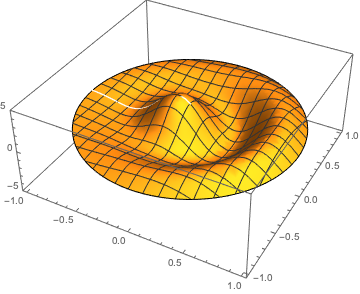
\includegraphics[width = 4.5 cm]{images/initialvalue.png}
  \caption{Initial distribution to be analyzed.}
\end{figure}
If we use this as the initial value of the heat equation, we have the following solution:
\begin{equation}
  u(r,\phi,t)=\frac{9}{4}J_0(\alpha_{03}r)e^{-\alpha_{03}^2 t}-3 J_1(\alpha_{12}r)\cos(\phi)e^{-\alpha_{12}^2 t}+\frac{1}{5} J_2(\alpha_{24}r)\sin(2\phi)e^{-\alpha_{12}^2 t}
\end{equation}
As we can see the components normal modes with larger eigenvalues will decay more quickly which is why the heat equation is so effective at "smoothing" surface. Below are some plots of the solution at later times.
\begin{figure}[H]
  \centering
  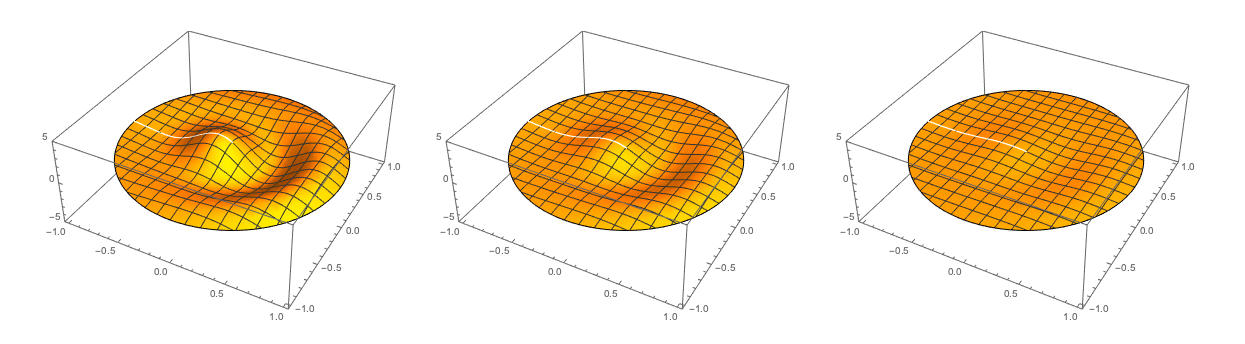
\includegraphics[width = 1.0\textwidth]{images/heat.png}
  \caption{Evolution of heat equation for initial distribution given.}
\end{figure}
If we use this as the initial displacement for the wave equation with no initial velocity, we see that the waves interact in interesting ways to produce the following effects.
\begin{equation}
    u(r,\phi,t)=\frac{9}{4}J_0(\alpha_{03}r)\cos(\alpha_{03} t)-3 J_1(\alpha_{12}r)\cos(\phi)\cos(\alpha_{12} t)+\frac{1}{5} J_2(\alpha_{24}r)\sin(2\phi)\cos(\alpha_{12} t)
\end{equation}
\begin{figure}[H]
  \centering
  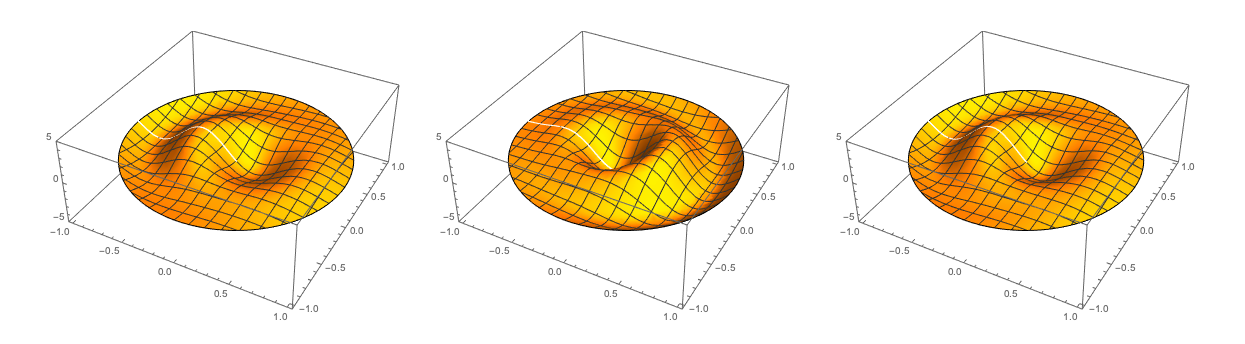
\includegraphics[width = 1.0\textwidth]{images/wave.png}
  \caption{Evolution of wave equation for initial displacement given.}
\end{figure}
We can also use this as the initial distribution for the velocity of the wave. In this case, the displacements are very minor, and we can see that there are only slight deviations from the at rest behavior.
\begin{equation}
    u(r,\phi,t)=\frac{9}{4 \alpha_{03}}J_0(\alpha_{03}r)\sin(\alpha_{03} t)-\frac{1}{\alpha_{12}} J_1(\alpha_{12}r)\cos(\phi)\sin(\alpha_{12} t)+\frac{1}{5\alpha_{24}} J_2(\alpha_{24}r)\sin(2\phi)\sin(\alpha_{12} t)
\end{equation}

\begin{figure}[H]
  \centering
  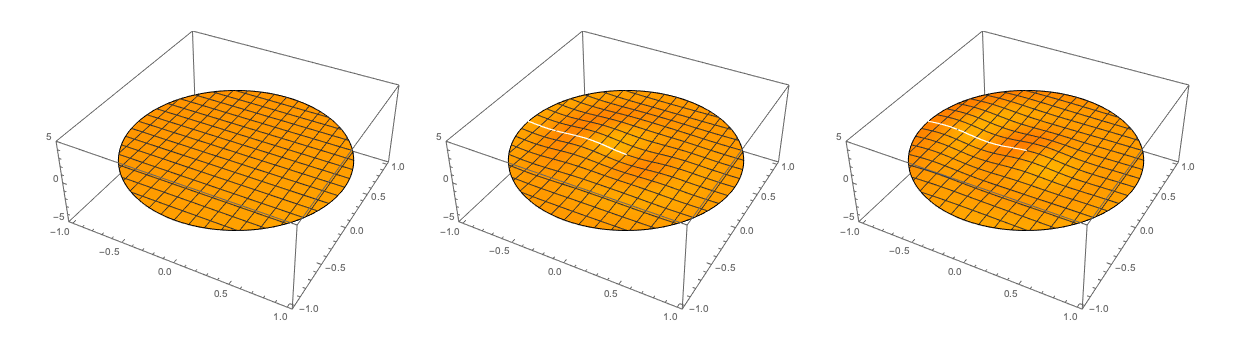
\includegraphics[width = 1.0\textwidth]{images/wavevel.png}
  \caption{Evolution of wave equation for initial velocity given.}
\end{figure}
We can see that these solutions to the heat equation are oscillating about the steady state solution $u = 0$. We also see that for the solution where only the initial velocity is given, the amplitude is much lower than it is when the initial displacement is given. This is because we are dividing each term of the solution by its corresponding eigenvalue. This in turn means that the initial velocity does not impact the dynamics as much as the initial position does.
\section{Conclusion}
Through the method of eigenfunction expansions, solutions to the heat and wave equation are generated, which in turn allow us to analyze the dynamics of solutions. We see that the wave equation is the higher dimensional analogue to the simple harmonic oscillator, and the heat equation is the higher dimensional analogue to exponential decay. Instead of the solutions oscillating or decaying towards an equilibrium point, they end up decaying to an equilibrium function, one that is harmonic.\\
It is important to reiterate that this method of solving functions by eigenfunction expansion is not unique to the Laplace operator, and can be used for any operator that satisfies equation (\ref{selfadjoint}), known as a self-adjoint operator. This allows us to in principal solve nearly any linear-homogenous PDE. In fact this method has a direct analogy to methods for solving a linear system of ODEs. Traditionally, we attempt to find the eigenvalues and straight-line solutions to the equation, which corresponds to finding the normal modes of a differential operator.
\newpage
\begin{appendices}
\section{Solutions to Laplace's Equation}
Given their importance in both the heat and wave equations, it is important to introduce some properties of solutions to Laplace's equation. The most important property of Laplace's equation is the averaging property. Suppose we have a function $u:\Omega\rightarrow\bb{R}$, then for all $x\in\Omega$, $u(x)$ is the average of the outputs of $u$ for all points an equal distance from $x$. This is a feature we will prove for the unit disc.\\
In order to solve Laplace's equation, we begin with separation of variables:
\begin{equation}
  \frac{1}{f(r)}\left[ r^2 \dder{^2 f}{r^2} + r\dder{f}{r} \right] =-\frac{1}{g(\phi)}\dder{^2 g}{\phi^2} = n^2
\end{equation}
Here the angular equation is the same as it was for the Helmholtz equation, however this time we express the solution in terms of sine and cosine functions
\begin{equation}
  g(\phi)=A_n \cos n\phi+B_n \sin n\phi
\end{equation}
The radial equation is slightly different now since we no longer have the eigenvalue term:
\begin{equation}
  r^2 f''+ r f'- n^2 f=0
\end{equation}
This is an Euler-Cauchy problem, and has solutions $r^{\pm n}$. Since we require the function to be at the very least continuous inside the unit disc, we only keep the $r^n$ term. This means that the general solution to Laplace's equation is:
\begin{equation}
  u(r,\phi)=\sum_{n=0}^\infty A_n r^n \cos n\phi + B_n r^n \sin n\phi
\end{equation}
For the boundary conditions we have worked with through this report, we specified the value of the function on the boundary, so our boundary contition is $u(1,\phi)= h(\phi)$. If we insert this into our solution we get:
\begin{equation}
  h(\phi) = \sum_{n=0}^\infty A_n \cos n\phi+B_n \sin n\phi
\end{equation}
This is the Fourier series in terms of sine and cosine functions. These form another basis for functions on the unit circle. If we rewrite the sine and cosine functions in terms of complex exponentials, we find the following relations between the expansion coefficients:
\begin{equation}
  \begin{matrix}
    A_o = 2 c_o\\
    A_n = c_n + c_{-n}\\
    B_n = i(c_n - c_{-n})
  \end{matrix}
\end{equation}
This allows us to write the expansion coefficients as:
\begin{equation}
  \begin{matrix}
    A_o = \frac{1}{2\pi}\int_0^{2\pi} u(1,\phi)d\phi\\
    A_n = \frac{1}{\pi}\int_0^{2\pi} u(1,\phi)\cos n\phi d\phi\\
    B_n = \frac{1}{\pi}\int_0^{2\pi} u(1,\phi)\sin n\phi d\phi\\
  \end{matrix}
\end{equation}
The solution $u(r,\phi)$ can be written in terms of a Green's function in the following way:
\begin{equation}P(r,\phi,\phi') = \frac{1}{2\pi}\left(1+ 2\sum_{n=1}^\infty r^n (\cos n\phi\cos n\phi'+\sin n\phi\sin n\phi') \right)
\end{equation}
Through this function, we may write the solution as:
\begin{equation}
  u(r,\phi) = \int_0^{2\pi} u(1,\phi')P(r,\phi,\phi')d\phi'
\end{equation}
Unlike the Green's functions for the wave or heat equations, this can be simplified greatly. We first make use of the identity $\cos(a-b)=\cos a\cos b+\sin a\sin b$, and then rewrite our cosine function in terms of complex exponentials,
\begin{equation}
  P(r,\phi,\phi') = \frac{1}{2\pi}\left(
    1+\sum_{n = 1}^{\infty } (re^{i(\phi-\phi')})^n + (re^{-i(\phi-\phi')})^n 
  \right)
\end{equation}
The geometric series tells us that:
\begin{equation}
  \sum_{n=0}^\infty x^n = 1+\sum_{n=1}^\infty x^n = \frac{1}{1-x}
\end{equation}
for $|x|<1$. Since $r\in [0,1]$ and the complex exponentials never exceed 1, we have convergence:
\begin{equation}
  P(r,\phi,\phi') = \frac{1}{2\pi}\left(1+\frac{1}{1-r \exp(i(\phi-\phi'))}-1 + \frac{1}{1-\exp(-i(\phi-\phi'))} - 1\right)
\end{equation}
This can be simplified to give:
\begin{equation}
  \boxed{
    P(r,\phi,\phi') = \frac{1}{2\pi} \frac{1-r^2}{1 - 2r \cos(\phi-\phi') - r^2}
  }
\end{equation}
This is known as the Poisson kernel, and allows us to write a general solution to Laplace's equation. If we consider the value of the function at $r=0$, we see that the value is:
\begin{equation}
  u(0,\phi) = \frac{1}{2\pi}\int_0^{2\pi} u(1,\phi)d\phi
\end{equation}
which confirms the averaging property of solutions to Laplace's equation.
\section{Inhomogenous Boundary Conditions}
Throughout this report, we used the boundary condition that the function must vanish at the boundary. However in certain situations, the boundary may be a non-zero function for all time. In the contex of the the heat equation, this means that the boundary is kept at a fixed temperature, and the solution will tend towards the solution to Laplace's equation with that boundary value. Suppose that for both the wave and heat equation, we have the restriction $u(1,\phi,t)=h(\phi)$. We will define a new function:
\begin{equation}
  v(r,\phi,t) = u(r,\phi,t) - \int_0^{2\pi} P(r,\phi,\phi')h(\phi')d\phi'
\end{equation}
where $P$ is the Poisson kernel. We see that $v$ is now zero at the boundary, and still will satisfy the wave or heat equation. We may now solve the initial value problem for $v(r,\phi,t)$ and then solve for $u(r,\phi,t)$. 
\end{appendices}
\newpage
\setcounter{secnumdepth}{0}
\section{References}
Asmar, N. H. (2002). \textit{Applied complex analysis with partial differential equations}. New Jersey: Prentice-Hall Inc.\\
\begin{adjustwidth}{2 cm}{}
This book was used to understand differential equations in polar and spherical coordinate systems, as well as certain properties of Bessel functions.\\
\end{adjustwidth}
Farlow, S. J. (2016). \textit{Partial differential equations for scientists and engineers}. New York: Dover Publications, Inc.\\
\begin{adjustwidth}{2 cm}{}
This book was used to understand the basic types of partial differential equations, as well as some methods for solving them in one dimension. It also introduced the physical interpretation of these equations.\\
\end{adjustwidth}
Fetter, A. L., \& Walecka, J. D. (2003). \textit{Theoretical mechanics of particles and continua}. Mineola, NY: Dover Publications. \\
\begin{adjustwidth}{2 cm}{}
This book was used to understand the physical meaning behind the wave and heat equation, as well as some theorems from Sturm-Liouville theory.\\
\end{adjustwidth}
Jackson, J. D. (1972). Classical electrodynamics (1st ed.). New York: Wiley.\\
\begin{adjustwidth}{2 cm}{}
This book was useful in introducing the method of eigenfunction expansions, Green's functions, and different types of boundary value problems.\\
\end{adjustwidth}
Tolstov, G. P. (2009). \textit{Fourier series}. New York: Dover Publications, Inc.\\
\begin{adjustwidth}{2 cm}{}
This book was used to understand basic properties of Fourier Series and Fourier-Bessel Series, as well as general methods of eigenfunction expansions.
\end{adjustwidth}
\end{document}
